\documentclass[11pt]{report}

\usepackage[utf8]{inputenc}
\usepackage[francais]{babel}
\usepackage[T1]{fontenc}
\usepackage{graphicx}

\title{ Projet LO41 : Les boucles de recompletement}
\author{Chiara \bsc{Salvoni} \& Romain \bsc{Thibaud}}
\date{Automne 2014}

\renewcommand{\contentsname}{Sommaire}

\begin{document}

\maketitle

\tableofcontents

\chapter{Introduction}

Ce projet a été réalisé dans le cadre d'un enseignement du département informatique de l'UTBM. Il a pour objectif de nous faire accuérir des connaissances en programmation orienté système. Le choix du langage C a été imposé afin qu'il ne soit question que d'une application à un nouveau problème des différentes notions abordées dans ce même langage dans le cadre des travaux pratiques. Ce projet constitue une traduction en langage informatique d'une méthode de production pratiquée dans le monde industriel : la méthode Kanban. 

Il est d'abord nécessaire de décrire concrètement en quoi consiste cette méthode et dans quelle mesure nous devons l'implémenter. 

S'en suit alors une analyse du problème posé afin d'y répondre aux mieux. Nous utlisons par exemple un réseau de pétri afin d'imager la problématique. 

Enfin il ne reste plus qu'à implémenter en C une solution en choisissant parmi les outils que nous avons vu en cours et s'organiser pour effectuer un travail à plusieurs.

\chapter{La méthode Kanban : description}

	\section{Description}
	
	La méthode Kanban est une méthode de production inventé par les ingénieurs de chez Toyota dans les années 50. Elle tranche avec les méthodes utilisées précédemment par sa volonté de réduire la quantité des stocks et donc de ne produire que le strict nécessaire. La production s'adapte donc à la consommation en temps réels. Cette vision de la production facilite un diversification des productions et rompt donc avec la standardisation engendré par des méthodes tel le Fordisme. Elle garde néammoins un aspect Tayloriste puisqu'elle continue de disséquer la fabrication du produit pour en optimiser le temps nécessaire à sa création.
	
	Cet outils de productions repose sur un système d'étiquettes (Kanban en japonnais) qui permet la synchronisation des différents postes entre eux. A la prise d'un conteneur plein de pièce, l'opérateur prend alors l'étiquette qui lui ait lié et l'ajoute à un conteneur vide. Un agent passe alors récupérer les containeur vides avec étiquette pour les transporter au poste où les pièces sont fabriquées. Le conteneur est alors rempli et ensuite réacheminé au premier poste.
	
	La force de cette méthode est son adaptativité aux besoins de consommations. Il est rapide et simple de changer un processus de fabrication sans que cela n'entraine de trop grosses pertes matérieles et temporelles. Cependant elle atteint ces limites du moment que l'on rencontre un problème sur la chaine de fabrication. En effet la défaillance d'un poste entraine l'arrêt de toute la production, c'est pourquoi en multipliant le nombre de postes on augmente les chances d'incidents et donc d'inactivté, ce qui implique une perte de temps dans le processus de fabrication.
	
	\section{Donnée du problème}
	
	L'objectif est donc, ici, de simuler le fonctionnement de ce processus de fabrication en langage C. Nous devons fournir une solution qui permet à un utilisateur de choisir un produit (c'est à dire un nombre de postes de travail) ainsi qu'un nombre de pièces et qui mime la chaine de production de ce produit. 
	
	Chaque poste devra travailller en collaboration avec les deux qui l'encadre (le poste amont et le poste aval) pour répondre au plus juste à la demande. Un poste ne pourra commencer sa production que s'il a eu une commande du poste en aval. Comme les stocks sont limités il ne pourra y avoir plus deux conteneurs pleins d'une même pièce. 
	
	De plus, pour assurer la propreté du programme, toutes les ressources devront être nettoyé que se soit lors d'un arrêt normal en fin de production ou dans le cas d'un interruption du programme.
\chapter{Analyse du problème}
	
	\section{Réseau de pétri}
	
	Afin de bien structurer notre pensée concernant le problème posé, nous avons établit un réseau de pétri représentant le fonctionnement d'un seul poste de travail :
	
	\begin{figure}[!h]
\centering
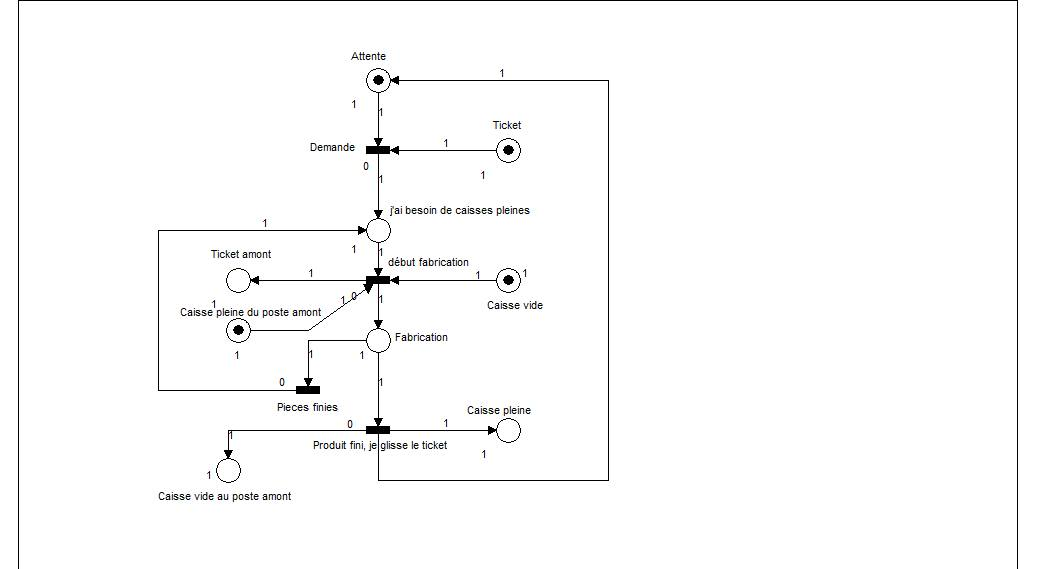
\includegraphics[width=16cm]{reseau.jpg}
\caption{Réseau de pétri : fonctionnement d'un poste de travail}
\end{figure}
	
	\section{Observations globales}
		De toute évidence chaque poste de travail est indépendant des autres. Il alimente la chaine avec ses pièces, mais travail en autonomie sur son produit. Il n'a de contact avec les autres postes que par l'intermédiaire des étiquettes et des conteneurs, qu'ils soient vides ou pleins. On voit alors facilement que les ressources partagées dans le programme sont les étiquettes et les caisses, et qu'elles seront manipulées par des agents qui seront les postes de travails. 
	
		
\chapter{Mis en \oe{}uvre}

	\section{Organisation}
	Nous avons donc été deux pour réaliser ce projet. Pour faciliter le travail ensemble nous avons mis en place un gestionnaire de version, à savoir git. Ce choix nous a permis de travailler ensemble sans se gêner et donc d'avancer à un rythme raisonnable. 
	
	Le language nous étant imposé, nous n'avons pas eu de choix a effectué, et nous n'avons pas jugé utile de se servir d'un IDE pour le dévellopement, la compilation en C étant simple depuis une distribution Linux et les outils de débogguage performant. Nous avons donc simplement utilisé un éditeur de text et une console. 
	
	Concernant la répartition du travail, nous avons préféré travailler ensemble sur chacune des fonctions plutôt que séparé le travail et rassembler le tout à la fin. Cela nous a permis d'avoir un regard critique sur les lignes de codes que l'on venait d'implémenter et surtout d'avoir une cohérence dans les technologies utilisées. 
	\section{Choix techniques}
	Afin d'assurer une indépendance des postes de travails et surtout la simultanéité de leur travail, deux choix s'offraient à nous : chaque poste un processus ou chaque poste est un thread. Nous avons optés pour la deuxième solution. Ce choix a été motivé par une volonté d'évolution. En effet dans l'éventualité où l'on souhaite simuler le fonctionnement d'une usine, avec donc plusieurs chaines de productions, on pourrait alors modeliser chaque chaine par un processus et donc chaque poste de travail par un thread. C'est dans cet optique que nous avons choisit d'utiliser des threads d'entrée pour modéliser nos postes de travail.
	
	Concernant les ressources partagées dans le programme nous avons décidé d'utiliser des sémaphores afin de les représenter. Ils permettent de synchroniser nos threads entre eux et donc de ne travailler que quand ils en ont le droits. Concrètement, nous avons trois tableaux de sémaphores que l'on alloue dynamiquement en fonction du nombre de postes afin d'économiser au plus les ressources de la machine. Plus concrètement, nous avons mis en place des sémaphores posix, car nous les trouvons plus agréable à manipuler et cela ne pose pas de problème comme nous dialoguons au sein d'un seul processus contenant plusieurs threads. 
	
	Pour la gestion de la libération de mémoire nous avons simplement choisit de "surcharger" le signal SIGSTOP (Ctrl+C). Son appel provoque la désallocation de toutes les variables dynamiques et autres threads. On rétablit alors la valeur par défaut du signal qui coupe alors l'éxecution du programme.
	
	\section{Que pourrait-on ajouter ?}
	
	Nous l'avons évoqué plutôt dans ce rapport, il y a la possibilité de simuler une usine fabriquant plusieurs produits en même temps en se servant de plusieurs processus. Il est possible de pousser le concept en ajoutant un même poste de travail à plusieurs chaines de productions. Par contre un tel changement implique par exemple de changer les sémaphores posix en sémaphores IPC, ou encore la mise en place de pipes pour la comminication inter-processus.
\chapter{Conclusion}
\begin{description}
\item[Retour de Chiara : ]Ce projet nous a permis de nous familiariser avec les threads et leurs utlisations, en traitant
un problème où la quantité de ces derniers peux etre parametrable.

C'était mon premier projet réalisé en langage C, et donc j'ai pu approfondir mes connaissances,
en essayant avec plusieurs solutions pour chercher celle qui permettait au mieux de répondre
au sujet proposé. De plus, j'ai appris à utiliser l'outil Github. Il a été très precieux dans notre
travail car il nous a permis d'échanger rapidement les informations entre nous.

J'ai apprécié le travail en équipe, une compétence qui peut etre utile dans notre future carrière.
\item[Retour de Romain : ]Pour moi, ce sujet fut une réelle surprise. J'avais de grandes appréhensions concernant l'intêret qu'il suciterait chez moi. Je me suis finalement pris au jeu dans un langage que je n'apprécie pas spécialement.

Cet aspect de gestion des ressources au plus près de la machine est au final très prenant et instructif concernant les comportements de certains programmes. 

Au final, l'aspect travaille en groupe est toujours très enrichissant. Il nous permet de découvrir d'autres vision des problèmes, et offre surtout une opportunité de mettre ses idées à l'épreuves et donc la possiblités de se remettre en cause, un avantage certain pour progresser.
\end{description}
\end{document}